%% abtex2-modelo-relatorio-tecnico.tex, v-1.9.6 laurocesar
%% Copyright 2012-2016 by abnTeX2 group at http://www.abntex.net.br/ 
%%
%% This work may be distributed and/or modified under the
%% conditions of the LaTeX Project Public License, either version 1.3
%% of this license or (at your option) any later version.
%% The latest version of this license is in
%%   http://www.latex-project.org/lppl.txt
%% and version 1.3 or later is part of all distributions of LaTeX
%% version 2005/12/01 or later.
%%
%% This work has the LPPL maintenance status `maintained'.
%% 
%% The Current Maintainer of this work is the abnTeX2 team, led
%% by Lauro César Araujo. Further information are available on 
%% http://www.abntex.net.br/
%%
%% This work consists of the files abntex2-modelo-relatorio-tecnico.tex,
%% abntex2-modelo-include-comandos and abntex2-modelo-references.bib
%%

% ------------------------------------------------------------------------
% ------------------------------------------------------------------------
% abnTeX2: Modelo de Relatório Técnico/Acadêmico em conformidade com 
% ABNT NBR 10719:2015 Informação e documentação - Relatório técnico e/ou
% científico - Apresentação
% ------------------------------------------------------------------------ 
% ------------------------------------------------------------------------

\documentclass[
	% -- opções da classe memoir --
	12pt,				% tamanho da fonte
	openany,			% capítulos começam em pág ímpar (insere página vazia caso preciso)
	twoside,			% para impressão em recto e verso. Oposto a oneside
	a4paper,			% tamanho do papel. 
	% -- opções da classe abntex2 --
	%chapter=TITLE,		% títulos de capítulos convertidos em letras maiúsculas
	%section=TITLE,		% títulos de seções convertidos em letras maiúsculas
	%subsection=TITLE,	% títulos de subseções convertidos em letras maiúsculas
	%subsubsection=TITLE,% títulos de subsubseções convertidos em letras maiúsculas
	% -- opções do pacote babel --
	english,			% idioma adicional para hifenização
	french,				% idioma adicional para hifenização
	spanish,			% idioma adicional para hifenização
	brazil,				% o último idioma é o principal do documento
	]{abntex2}


% PACOTES

% ---
% Pacotes fundamentais 
\usepackage{lmodern}			% Usa a fonte Latin Modern
\usepackage[brazil]{babel}
\usepackage{amsmath,amsfonts,amsthm,amstext,amssymb}
\usepackage[T1]{fontenc}		% Selecao de codigos de fonte.
\usepackage[utf8]{inputenc}		% Codificacao do documento (conversão automática dos acentos)
\usepackage{indentfirst}		% Indenta o primeiro parágrafo de cada seção.
\usepackage{color}				% Controle das cores
\usepackage{graphicx}			% Inclusão de gráficos
\usepackage{microtype} 			% para melhorias de justificação
% ---

% Pacotes adicionais, usados no anexo do modelo de folha de identificação
\usepackage{multicol}
\usepackage{multirow}
\usepackage{float} % para utilizar o H de tabelas e figuras e mante-las no lugar
% ---

%----------------- PARA INSERIR ARQUIVOS DE CODIGOS -----------------%
\usepackage[dvipsnames]{xcolor}% Definindo novas cores
\definecolor{verde}{rgb}{0,0.5,0}
% Configurando layout para mostrar codigos C++
\usepackage{courier}
\DeclareUnicodeCharacter{2212}{-}



%\lstset { %
%    language=C++,
%    basicstyle=\footnotesize\ttfamily,% basic font setting
%}
\usepackage{pythonhighlight}
\lstset{ %
  backgroundcolor=\color{white},   % choose the background color; you must add \usepackage{color} or \usepackage{xcolor}
  basicstyle=\footnotesize,        % the size of the fonts that are used for the code
  breakatwhitespace=false,         % sets if automatic breaks should only happen at whitespace
  breaklines=true,                 % sets automatic line breaking
  captionpos=b,                    % sets the caption-position to bottom
  commentstyle=\color{OliveGreen}\textit,    % comment style
  deletekeywords={...},            % if you want to delete keywords from the given language
  escapeinside={\%*}{*)},          % if you want to add LaTeX within your code
  extendedchars=true,              % lets you use non-ASCII characters; for 8-bits encodings only, does not work with UTF-8
  frame=single,	                   	   % adds a frame around the code
  keepspaces=true,                 % keeps spaces in text, useful for keeping indentation of code (possibly needs columns=flexible)
  keywordstyle=\color{blue}\bfseries,       % keyword style
  language=C++,                 % the language of the code (can be overrided per snippet)
  otherkeywords={*,fopen,fclose,fprintf},           % if you want to add more keywords to the set
  numbers=left,                    % where to put the line-numbers; possible values are (none, left, right)
  numbersep=5pt,                   % how far the line-numbers are from the code
  numberstyle=\tiny\color{black}, % the style that is used for the line-numbers
  rulecolor=\color{black},         % if not set, the frame-color may be changed on line-breaks within not-black text (e.g. comments (green here))
  showspaces=false,                % show spaces everywhere adding particular underscores; it overrides 'showstringspaces'
  showstringspaces=false,          % underline spaces within strings only
  showtabs=false,                  % show tabs within strings adding particular underscores
  stepnumber=1,                    % the step between two line-numbers. If it's 1, each line will be numbered
  stringstyle=\color{BurntOrange}, % string literal style
  tabsize=2,	                   % sets default tabsize to 2 spaces
  title=\lstname,                  % show the filename of files included with \lstinputlisting; also try caption instead of title
  columns=fixed                    % Using fixed column width (for e.g. nice alignment)
}% -----------------% FIM INSERIR ARQUIVOs DE CODIGO -----------------%

% Pacotes de citações
\usepackage[brazilian,hyperpageref]{backref}	 % Paginas com as citações na bibl
\usepackage[num]{abntex2cite}	% Citações padrão ABNT
\citebrackets() %citação numérica entre colchetes
% --- 


% CONFIGURAÇÕES DE PACOTES

% Configurações do pacote backref
% Usado sem a opção hyperpageref de backref
\renewcommand{\backrefpagesname}{Citado na(s) página(s):~}
% Texto padrão antes do número das páginas
\renewcommand{\backref}{}
% Define os textos da citação
\renewcommand*{\backrefalt}[4]{
	\ifcase #1 %
		Nenhuma citação no texto.%
	\or
		Citado na página #2.%
	\else
		Citado #1 vezes nas páginas #2.%
	\fi}%
% ---


% Informações de dados para CAPA e FOLHA DE ROSTO
\titulo{Lista 3 - Controle de Sistemas Dinâmicos\\Derivada e Integral Numérica}
\autor{Frederico José Ribeiro Pelogia} %NAO PREENCHER
\local{São José dos Campos - Brasil}
\data{Dezembro de 2020}
\instituicao{
  Docente: Prof. Dr. Henrique Mohallem Paiva
  \par
  Universidade Federal de São Paulo - UNIFESP
  \par
  Instituto de Ciência e Tecnologia - Campus São José dos Campos
}
\tipotrabalho{Relatório técnico}
\preambulo{Relatório apresentado à Universidade Federal de São Paulo como parte dos requisitos para aprovação na disciplina Controle de Sistemas Dinâmicos}
% ---

% Configurações de aparência do PDF final

% alterando o aspecto da cor azul
\definecolor{blue}{RGB}{41,5,195}

% informações do PDF
\makeatletter
\hypersetup{
     	%pagebackref=true,
		pdftitle={\@title}, 
		pdfauthor={\@author},
    	pdfsubject={\imprimirpreambulo},
	    pdfcreator={LaTeX with abnTeX2},
		pdfkeywords={abnt}{latex}{abntex}{abntex2}{relatório técnico}, 
		colorlinks=true,       		% false: boxed links; true: colored links
    	linkcolor=blue,          	% color of internal links
    	citecolor=blue,        		% color of links to bibliography
    	filecolor=magenta,      		% color of file links
		urlcolor=blue,
		bookmarksdepth=4
}
\makeatother
% --- 
% Espaçamentos entre linhas e parágrafos 

% O tamanho do parágrafo é dado por:
\setlength{\parindent}{1.3cm}

% Controle do espaçamento entre um parágrafo e outro:
\setlength{\parskip}{0.2cm}  % tente também \onelineskip

% compila o indice
\makeindex
% ---



% ------------------------------------------------
% Início do documento
\begin{document}

% Seleciona o idioma do documento (conforme pacotes do babel)
%\selectlanguage{english}
\selectlanguage{brazil}

% Retira espaço extra obsoleto entre as frases.
\frenchspacing 

% ----------------------------------------------------------
% ELEMENTOS PRÉ-TEXTUAIS
% ----------------------------------------------------------
% \pretextual

% ---
% Capa
\imprimircapa
% ---

% ---
% Folha de rosto
\imprimirfolhaderosto*
% ---

% ---
% RESUMO
% resumo na língua vernácula (obrigatório)
%\setlength{\absparsep}{18pt} % ajusta o espaçamento dos parágrafos do resumo
%\begin{resumo}


% \noindent
% \textbf{Palavras-chaves}: Processador, Arquitetura e Organização de Computadores, Verilog, Unidade de Processamento, Unidade de Controle.
%\end{resumo}

%------LISTAS SÃO OPCIONAIS---------
% inserir lista de ilustrações
%\pdfbookmark[0]{\listfigurename}{lof}
%\listoffigures*
%\clearpage


% inserir lista de tabelas
%\pdfbookmark[0]{\listtablename}{lot}
%\listoftables*
%\clearpage
% ---

% inserir lista de listings
%\pdfbookmark[0]{\listlisingsname}{lol}
%\lstlistoflistings
%\clearpage

%SUMÁRIO É OBRIGATÓRIO
% inserir o sumario
\pdfbookmark[0]{\contentsname}{toc}
\tableofcontents*
% ---


% ----------------------------------------------------------
% ELEMENTOS TEXTUAIS
\textual

% ----------------------------------------------------------
\chapter{Introdução}
Sistemas  dinâmicos podem ser descritos por uma ou mais equações diferenciais, que podem ser complexas demais para serem solucionadas analiticamente. Dessa forma, para criar modelos e simulações para esse tipo de sistema, são recomendadas técnicas de integração numérica. 

O propósito desse relatório é investigar a preferência pela integração numérica em relação à derivação numérica, quando tratando-se de situações com ruído, que sempre estarão presentes em problemas reais. Os testes realizados utilizarão o Método de Euler, que apresenta uma forma simples, mas razoável, de tratar equações diferenciais computacionalmente \cite{paulnotes}.

O método e as simulações serão implementados na linguagem de programação C e os dados, salvos em um arquivo de texto. Para a criação dos gráficos a partir dos dados será utilizada a liguagem de programação Python, com a biblioteca gráfica \pyth{matplotlib}.

\chapter{Desenvolvimento}
\section{Código com os cálculos}
Primeiramente será apresentado o código na íntegra e depois serão comentadas as etapas para sua construção e será detalhado seu funcionamento.
\subsection{Código na íntegra}
O código que realiza os cálculos das derivadas e integrais está apresentado no Listing \ref{lst:ccode}.

\begin{lstlisting}[language=C++,caption={Código em C para cálculo das derivadas e integrais},captionpos=t,label=lst:ccode]
#include<stdio.h>
#include<stdlib.h>
#include<math.h>

// Funcao que gera uma distribuicao normal
float * normal_dist(int n, float step, float mean, float std){
    // numero de termos: n / step 
    // media: mean
    // desvio padrao: std
    int i;
    float *nvec;
    nvec = malloc((n/step) * sizeof(float)); 
    for(i = 0; i < n/step ; i++){
        nvec[i] = exp(-0.5*pow((i*step - mean)/std, 2))/(std*sqrt(2*M_PI));
    }
    return nvec;
}

int main(int argc, char* argv[]){
    // Declarando variaveis importantes
    int i,t_max = 5;
    float *t, *y,*yd_ref, *yi_ref, *yd, *z, *zd, *zi,*noise,  step = 0.01, offset = 0;

    // Abrindo arquivo de texto para escrita
    FILE* fdata = fopen("data.txt","w");
    
    // Recebendo argumentos pela linha de comando
    if(argc > 1){
        t_max = atoi(argv[1]);
        step = atof(argv[2]);
        offset = atof(argv[3]);
    }
    
    // Alocando memoria para as variaveis
    t = malloc((t_max/step) * sizeof(float));
    y = malloc((t_max/step) * sizeof(float));
    yd_ref = malloc((t_max/step) * sizeof(float));
    yi_ref = malloc((t_max/step) * sizeof(float));
    yd = malloc((t_max/step) * sizeof(float));
    z = malloc((t_max/step) * sizeof(float));
    zd = malloc((t_max/step) * sizeof(float));
    zi = malloc((t_max/step) * sizeof(float));

    // Vetor com distribuicao normal de media 0 e desvio padrao 0.2
    noise = normal_dist(t_max, step, 0, 0.2);
    
    //Valores iniciais para y, sua derivada e sua integral 
    y[0] = 0;
    zd[0] = 0;
    zi[0] = 0;
    

    // loop principal pelos instantes de tempo
    for(i = 1; i < t_max/step; i++){
        //t: vetor com os instantes de tempo
        t[i] = i*step - offset;

        //y: y(t) = t^2
        y[i] = pow(t[i],2);

        //yd_ref: derivada teorica de y
        yd_ref[i] = 2*t[i];
        
        //yi_ref: integral teorica de y
        yi_ref[i] = pow(t[i],3)/3;

        //yd: derivada numerica de y (Metodo de Euler)
        yd[i] = (y[i] - y[i-1])/step;

        //z: z(t) = y(t) + ruido branco gaussiano
        z[i] = y[i] + noise[rand()% (int) (t_max/step)]; // amostra aleatoria da distr. normal
        
        //zd: derivada numerica de y com ruido (Metodo de Euler)
        zd[i] = (z[i] - z[i-1])/step;

        //zd: derivada numerica de y com ruido (Metodo de Euler)
        zi[i] = zi[i-1] + z[i]*step;

        // Gravando os dados no arquivo de texto
        fprintf(fdata, "%f %f %f %f %f %f %f %f\n", t[i], y[i], yd[i], yd_ref[i], yi_ref[i], z[i], zd[i], zi[i]);
    }

    // fechando arquivo de texto
    fclose(fdata);

    // desalocando as variaveis
    free(t);
    free(y);
    free(yd_ref);
    free(yi_ref);
    free(yd);
    free(z);
    free(zd);
    free(zi);
    free(noise);

    return 0;
}\end{lstlisting}
Pode-se perceber que o código inicia com a declaração e a alocação das variáveis necessárias, além da definição de alguns valores iniciais. Em seguida, é criado um loop principal que itera pelos instantes de tempo, populando os vetores e fazendo a escrita em um arquivo de texto de saída. Após isso, o arquivo de saída é fechado e as variáveis são desalocadas. 

Uma maneira muito mais eficiente, em termos de memória, de se escrever o código seria armazenar apenas o valor das variáveis no tempo presente e no imediatamente anterior. Entretanto, armazenar o histórico completo das variáveis, como foi feito no código, poderia ser interessante caso processamentos mais elaborados fossem necessários.

\subsection{Variáveis básicas}
As variáveis \emph{t, y, yd\_ref, yi\_ref} são essenciais para o presente relatório. 
\begin{itemize}
    \item A variável \emph{t} é um vetor com os instantes de tempo de $0$ a $5$ segundos com passo $0.01$, representando uma amostragem a cada $10\ ms$. Note, na linha 56 do Listing \ref{lst:ccode}, que é definido um \textit{offset} opcional, inicializado como 0 por padrão.
\item A variável \emph{y} é um vetor em que cada elemento na posição i recebe o valor de $(t[i])^2$, representando a função $y(t) = t^2$. 
\item As variáveis \emph{yd\_ref} e \emph{yi\_ref}, são vetores que possuem na posição i, respectivamente, $2t[i]$ e $\frac{(t[i])^3}{3}$, representando a derivada e a integral da função $y(t)$. É interessante notar que essas duas variáveis assumem conhecimento da derivada e da integral teóricas da função $y(t)$. Isso ocorre pois elas serão utilizadas como referência para avaliar o desempenho das aproximações numéricas.
\end{itemize}

\subsection{Derivada numérica sem ruído}
A variável \emph{yd} é um vetor que recebe, na posição i, 
$$y_d[i] = \frac{y[i] - y[i-1]}{\Delta t},$$
que é o valor da derivada numérica da função $y(t)$ no instante $t = t[i]$, utilizando a aproximação do Método de Euler.

\subsection{Adição de ruído}
Para a adição de um ruído branco gaussiano à variável y, foram realizadas as seguintes etapas:
\begin{itemize}
    \item Criação de uma função que retorna um vetor com uma distribuição normal com média $\mu$ e desvio padrão $\sigma$. A função criada foi a \emph{normal\_dist}, cuja definição está entre as linhas 6 a 17 do Listing \ref{lst:ccode}. A função de densidade de probabilidade utilizada como base \cite{normalwiki} foi $$\large f(x) = \frac{1}{\sigma \sqrt{2\pi}}e^{-\frac{1}{2}\left(\frac{x - \mu}{\sigma}\right)^2}.$$
    \item Chamada da função para criação de um vetor \emph{noise} com uma distribuição normal de média $0$ e desvio padrão $0.2$. 
    \item Criação da variável \emph{z} que possui, na posição i, o valor de $y[i]$ somado com uma \textbf{amostra aleatória} do vetor \emph{noise}. A amostra aleatória é retirada calculando-se um índice através do resto da divisão de um número aleatório pelo número de elementos do vetor, como pode se observar na linha 71 do Listing \ref{lst:ccode}. 
\end{itemize}

\subsection{Derivada numérica com ruído}
A variável \emph{zd} é um vetor que recebe, na posição i,
$$z_d[i] = \frac{z[i] - z[i-1]}{\Delta t},$$
que é o valor da derivada numérica da função $z(t)$ no instante $t = t[i]$, utilizando a aproximação do Método de Euler.

\subsection{Integral numérica com ruído}
A variável \emph{yd} é um vetor que recebe, na posição i,
$$z_i[i + 1] = z_i[i] + \Delta t z[i],$$
que é o valor da integral numérica da função $z(t)$ no instante $t = t[i]$, utilizando a aproximação do Método de Euler.

\section{Código para geração dos gráficos}
Para a criação dos gráficos a partir dos dados salvos no arquivo de texto, foi escrito um código em Python utilizando a bilbioteca gráfica \pyth{matplotlib}. O código está apresentado no Listing \ref{lst:pycode}.

\begin{lstlisting}[frame=none,caption={Código Python para geração dos gráficos.},captionpos=t,label=lst:pycode]
\end{lstlisting}
\begin{python}
import matplotlib.pyplot as plt

t = []
y = []
yd = []
yd_ref = []
yi_ref = []
z = []
zd = []
zi = []

# Abertura do arquivo com os dados
with open('data.txt','r') as f:
    # Leitura linha a linha do arquivo
    for line in f.readlines():
        values = line[:-1].split() # separacao das colunas
        # guardando os valores nas listas
        t.append(float(values[0]))
        y.append(float(values[1]))
        yd.append(float(values[2]))
        yd_ref.append(float(values[3]))
        yi_ref.append(float(values[4]))
        z.append(float(values[5]))
        zd.append(float(values[6]))
        zi.append(float(values[7]))

# Criacao dos graficos
fig, axs = plt.subplots(1, 2, figsize=(14,4))
fig.suptitle('Derivada sem ruido')
axs[0].plot(t, y)
axs[0].set(xlabel='t(s)', ylabel='Funcao y = x^2')
axs[0].grid()
axs[1].plot(t,yd, label='Numerica')
axs[1].set(xlabel='t(s)', ylabel='Derivada de y(t)')
axs[1].plot(t,yd_ref, label='Teorica')
axs[1].grid()
axs[1].legend()

fig, axs = plt.subplots(figsize=(10,5))
fig.suptitle('Adicao de ruido')
axs.plot(t, y, label='y(t) = x^2',zorder=2)
axs.set(xlabel='t(s)', ylabel='Funcao y(t) e z(t)')
axs.plot(t,z, label='z(t) = y(t) + ruido',zorder=1)
axs.grid()
axs.legend()

fig, axs = plt.subplots(1, 2, figsize=(14,4))
fig.suptitle('Derivada com ruido')
axs[0].plot(t, z)
axs[0].set(xlabel='t(s)', ylabel='Funcao z = x^2 + ruido')
axs[0].grid()
axs[1].plot(t,zd, label='Numerica com ruido (dz/dt Metodo de Euler)')
axs[1].set(xlabel='t(s)', ylabel='Derivada')
axs[1].plot(t,yd_ref, label='Teorica sem ruido (dy/dt)')
axs[1].grid()
axs[1].legend()

fig, axs = plt.subplots(1,2, figsize=(14,4))
fig.suptitle('Integral com ruido')
axs[0].plot(t, z)
axs[0].set(xlabel='t(s)', ylabel='Funcao z = x^2 + ruido')
axs[0].grid()
axs[1].plot(t,zi, label='Integral Numerica com ruido (Metodo de Euler)')
axs[1].set(xlabel='t(s)', ylabel='Integral')
axs[1].plot(t,yi_ref, label='Integral Teorica sem ruido')
axs[1].grid()
axs[1].legend()

plt.show()
\end{python}

Para a execução dos dois códigos em conjunto, foi criado o script \emph{run.sh}, apresentado no Listing \ref{lst:sh}.
\begin{lstlisting}[frame=none,caption={Script para execução dos códigos produzidos.},captionpos=t,label=lst:sh]
#!/bin/bash
gcc deriv_int.c -o di -lm 
./di 5 0.01 0
python plot.py
\end{lstlisting}


\chapter{Resultados e Discussões}

\section{Derivada sem ruído}
A Figura \ref{fig:yd} apresenta o gráfico de $y(t)$ e um gráfico que compara \emph{yd} com \emph{yd\_ref}, isto é, a aproximação numérica com o valor teórico da derivada.
\begin{figure}[H]
\center
    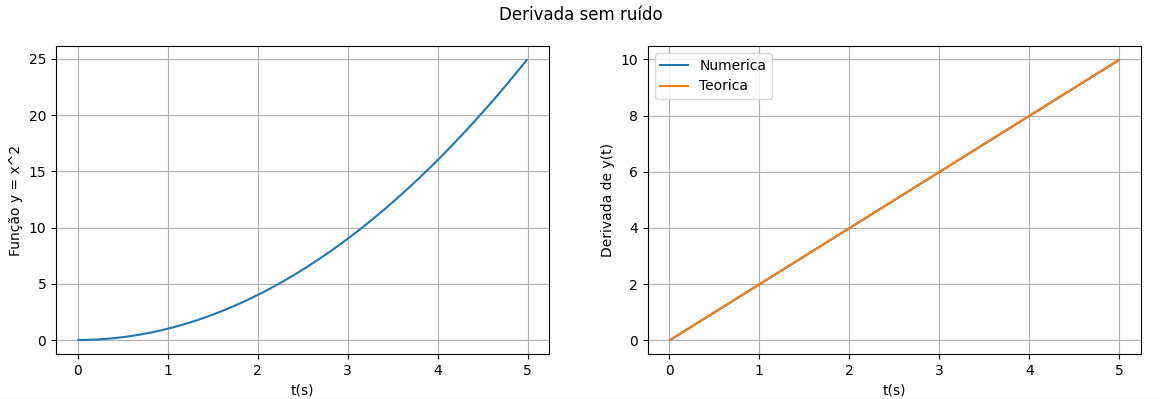
\includegraphics [scale = 0.5]{Figures/yd.png}
    \caption{Gráfico da função $y(t)$ e de suas derivadas teórica e numérica. Fonte: Autor}
    \label{fig:yd}
\end{figure}
Percebe-se que, sem a presença de ruído, as curvas da derivada teórica e da numérica estão sobrepostas, indicando que a aproximação foi bem sucedida e praticamente exata.

\section{Adição de ruído}
A Figura \ref{fig:z} apresenta um gráfico que compara a função $y(t)$ e sua versão $z(t)$, que apresenta a adição de ruído.
\begin{figure}[H]
\center
    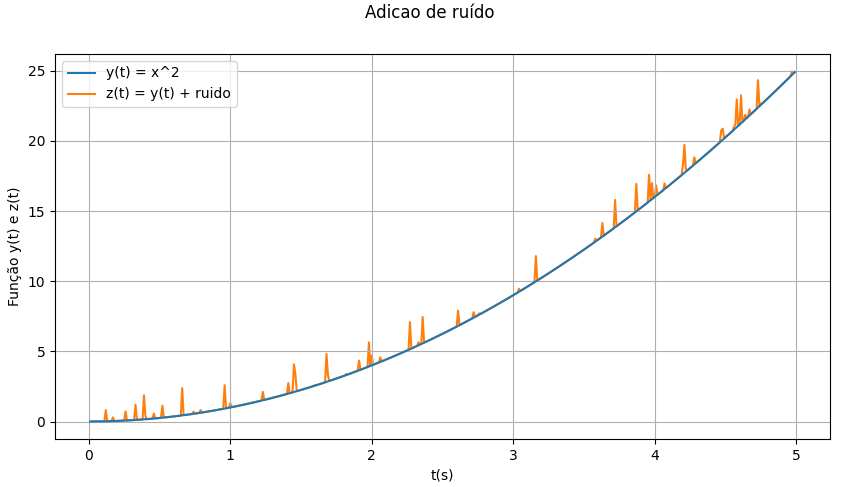
\includegraphics [scale = 0.5]{Figures/z.png}
    \caption{Gráficos das funções $y(t) = t^2$ e $z(t) = y(t) + \text{ruído}$. Fonte: Autor}
    \label{fig:z}
\end{figure}
Nota-se que o ruído adicionado gera alguns pequenos picos na curva original de $y(t)$. O procedimento para adição do ruído foi abordado no Capítulo de Desenvolvimento.

\section{Derivada com ruído}
A Figura \ref{fig:zd} apresenta o gráfico da função $z(t)$ e um gráfico que compara a derivada teórica de $y(t)$ com a aproximação pelo método de Euler da derivada de $z(t)$.
\begin{figure}[H]
\center
    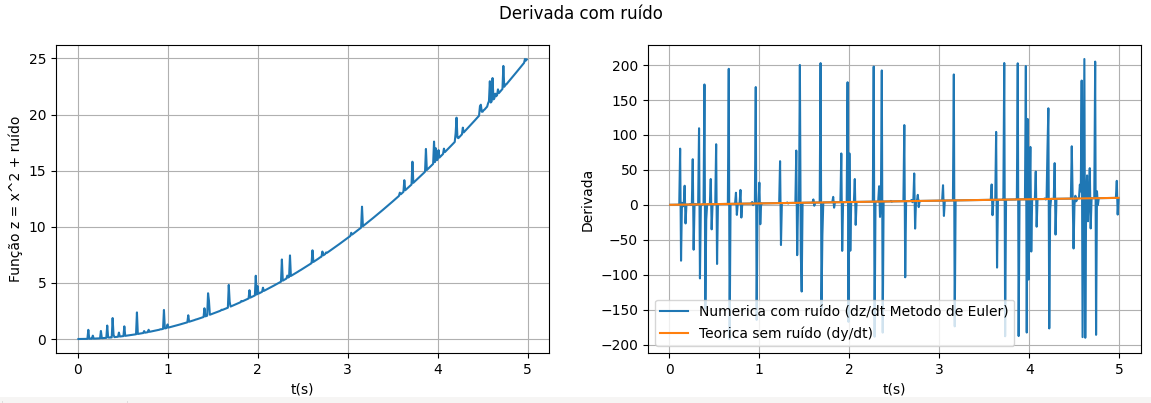
\includegraphics [scale = 0.5]{Figures/zd.png}
    \caption{Gráfico da função $z(t)$ e uma comparação de sua derivada numérica com a teórica de $y(t)$. Fonte: Autor}
    \label{fig:zd}
\end{figure}
Nota-se que, mesmo que pequeno, o ruído fez com que a derivda numérica ficasse extremamente imprecisa, atingindo valores muito diferentes dos esperados pela derivada teórica.

\section{Integral com ruído}
A Figura \ref{fig:zi} apresenta o gráfico da função $z(t)$ e um gráfico que compara a integral teórica da função $y(t)$ com a integral numérica, pelo Método de Euler, de $z(t)$.
\begin{figure}[H]
\center
    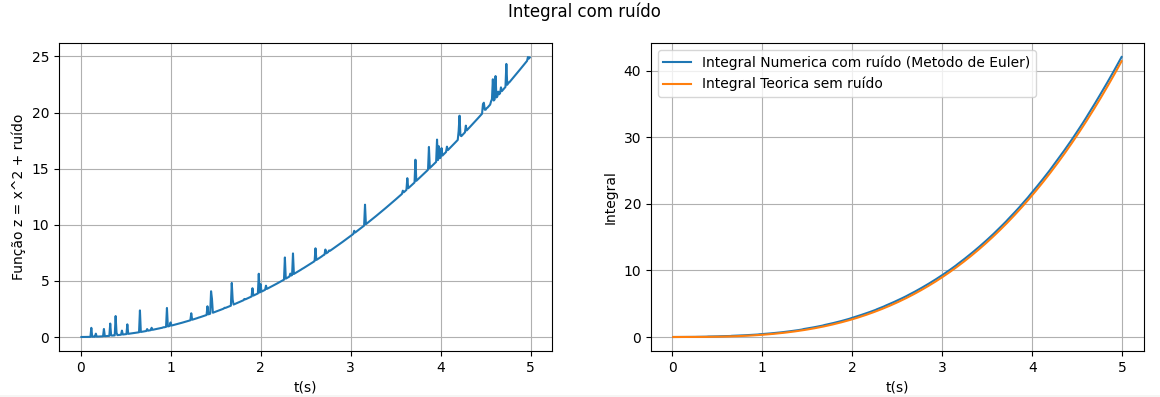
\includegraphics [scale = 0.5]{Figures/zi.png}
    \caption{Gráfico da função $z(t)$ e uma comparação de sua integral numérica com a teórica de $y(t)$. Fonte: Autor}
    \label{fig:zi}
\end{figure}
Percebe-se que, diferentemente da derivada numérica, a integral numérica apresentou uma boa aproximação para seu valor teórico, dado que as curvas estão quase sobrepostas na Figura \ref{fig:zi}. Essa robustez para lidar com ruído é o principal motivo da utilização de integradores em simulações numéricas de EDOs, em detrimento de derivadores.

\chapter{Considerações Finais}
Assim, os códigos escritos e os testes realizados foram sufientes para notar que a derivação numérica é muito mais sensível e menos robusta à presença de ruído do que a integração numérica. Isso motiva a preferência pela utilização de integradores à derivadores para simulações computacionais de sistemas dinâmicos e equações diferenciais.

% ---
% Finaliza a parte no bookmark do PDF
% para que se inicie o bookmark na raiz
% e adiciona espaço de parte no Sumário
% ---
%\phantompart


% ----------------------------------------------------------
% ELEMENTOS PÓS-TEXTUAIS
% ----------------------------------------------------------
\postextual

% ----------------------------------------------------------
% Referências bibliográficas
% ----------------------------------------------------------
\bibliography{ref} 
------------------------------


%---------------------------------------------------------------------
% INDICE REMISSIVO
%---------------------------------------------------------------------

\phantompart

\printindex


\end{document}
